


\tikzset{every picture/.style={line width=0.75pt}} %set default line width to 0.75pt        

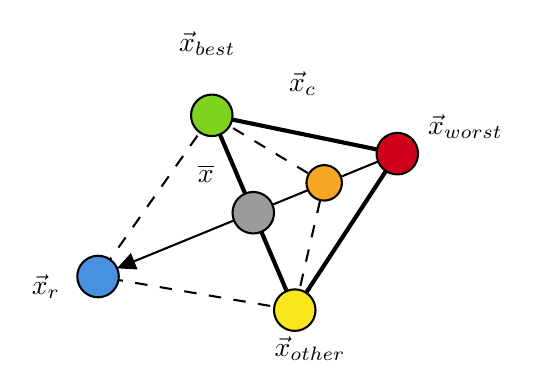
\begin{tikzpicture}[x=0.75pt,y=0.75pt,yscale=-1,xscale=1]
%uncomment if require: \path (0,914); %set diagram left start at 0, and has height of 914

%Straight Lines [id:da4445133148332976] 
\draw [line width=1.5]    (129.21,515.73) -- (218.59,534.19) ;
%Straight Lines [id:da8072652131616453] 
\draw [line width=1.5]    (169.18,609.58) -- (129.21,515.73) ;
%Straight Lines [id:da26520550089423445] 
\draw [line width=1.5]    (169.18,609.58) -- (218.59,534.19) ;
%Straight Lines [id:da04667789058155303] 
\draw    (218.59,534.19) -- (86.35,588.27) ;
\draw [shift={(83.58,589.41)}, rotate = 337.75] [fill={rgb, 255:red, 0; green, 0; blue, 0 }  ][line width=0.08]  [draw opacity=0] (8.93,-4.29) -- (0,0) -- (8.93,4.29) -- cycle    ;
%Shape: Circle [id:dp13626854632058039] 
\draw  [fill={rgb, 255:red, 155; green, 155; blue, 155 }  ,fill opacity=1 ] (139.99,566.57) .. controls (137.83,561.49) and (140.2,555.62) .. (145.28,553.45) .. controls (150.36,551.29) and (156.23,553.65) .. (158.4,558.74) .. controls (160.56,563.82) and (158.19,569.69) .. (153.11,571.85) .. controls (148.03,574.02) and (142.16,571.65) .. (139.99,566.57) -- cycle ;
%Shape: Circle [id:dp1389172126099203] 
\draw  [fill={rgb, 255:red, 208; green, 2; blue, 27 }  ,fill opacity=1 ] (209.39,538.1) .. controls (207.22,533.02) and (209.59,527.15) .. (214.67,524.99) .. controls (219.75,522.82) and (225.62,525.19) .. (227.79,530.27) .. controls (229.95,535.35) and (227.59,541.22) .. (222.51,543.39) .. controls (217.43,545.55) and (211.55,543.19) .. (209.39,538.1) -- cycle ;
%Straight Lines [id:da9263850358947512] 
\draw  [dash pattern={on 4.5pt off 4.5pt}]  (169.18,609.58) -- (74.4,593.39) ;
%Straight Lines [id:da334078503397518] 
\draw  [dash pattern={on 4.5pt off 4.5pt}]  (129.21,515.73) -- (74.4,593.39) ;
%Shape: Circle [id:dp17305345317593535] 
\draw  [fill={rgb, 255:red, 74; green, 144; blue, 226 }  ,fill opacity=1 ] (83.58,589.41) .. controls (85.77,594.47) and (83.45,600.36) .. (78.38,602.56) .. controls (73.32,604.76) and (67.43,602.43) .. (65.23,597.37) .. controls (63.03,592.3) and (65.36,586.41) .. (70.42,584.21) .. controls (75.49,582.01) and (81.38,584.34) .. (83.58,589.41) -- cycle ;
%Straight Lines [id:da5749691409395861] 
\draw  [dash pattern={on 4.5pt off 4.5pt}]  (169.18,609.58) -- (183.36,548.27) ;
%Straight Lines [id:da9253197524181758] 
\draw  [dash pattern={on 4.5pt off 4.5pt}]  (129.21,515.73) -- (183.36,548.27) ;
%Shape: Circle [id:dp59696029177814] 
\draw  [fill={rgb, 255:red, 126; green, 211; blue, 33 }  ,fill opacity=1 ] (120.01,519.65) .. controls (117.85,514.57) and (120.21,508.7) .. (125.29,506.53) .. controls (130.37,504.37) and (136.25,506.73) .. (138.41,511.81) .. controls (140.57,516.9) and (138.21,522.77) .. (133.13,524.93) .. controls (128.05,527.1) and (122.17,524.73) .. (120.01,519.65) -- cycle ;
%Shape: Circle [id:dp8536947286133791] 
\draw  [fill={rgb, 255:red, 248; green, 231; blue, 28 }  ,fill opacity=1 ] (159.98,613.49) .. controls (157.82,608.41) and (160.18,602.54) .. (165.26,600.38) .. controls (170.34,598.21) and (176.22,600.58) .. (178.38,605.66) .. controls (180.54,610.74) and (178.18,616.61) .. (173.1,618.78) .. controls (168.02,620.94) and (162.14,618.58) .. (159.98,613.49) -- cycle ;
%Shape: Circle [id:dp9385455494879282] 
\draw  [fill={rgb, 255:red, 245; green, 166; blue, 35 }  ,fill opacity=1 ] (175.51,551.61) .. controls (173.66,547.28) and (175.68,542.26) .. (180.02,540.41) .. controls (184.35,538.56) and (189.37,540.58) .. (191.22,544.92) .. controls (193.06,549.26) and (191.05,554.28) .. (186.71,556.12) .. controls (182.37,557.97) and (177.35,555.95) .. (175.51,551.61) -- cycle ;

% Text Node
\draw (112,474) node [anchor=north west][inner sep=0.75pt]   [align=left] {$\displaystyle \vec{x}_{best}$};
% Text Node
\draw (232,514) node [anchor=north west][inner sep=0.75pt]   [align=left] {$\displaystyle \vec{x}_{worst}$};
% Text Node
\draw (158,621) node [anchor=north west][inner sep=0.75pt]   [align=left] {$\displaystyle \vec{x}_{other}$};
% Text Node
\draw (121,538) node [anchor=north west][inner sep=0.75pt]   [align=left] {$\displaystyle \overline{x}$};
% Text Node
\draw (41,591) node [anchor=north west][inner sep=0.75pt]   [align=left] {$\displaystyle \vec{x}_{r}$};
% Text Node
\draw (165,493) node [anchor=north west][inner sep=0.75pt]   [align=left] {$\displaystyle \vec{x}_{c}$};


\end{tikzpicture}